\documentclass[PROP_AGutteridge_CS.tex]{subfiles}
\begin{document}

\chapter{Objectives}
The aims as outlined previously will be achieved by a comprehensive approach that both processes data and presents it in an alternative style. Figure 5 shows the proposed set of scenarios that the system will support, and that the system architecture choices will be based upon. This system will be designed to be compatible with modern browsers as its eventual use case, but will be developed and showcased as a local application for proof-of-concept. The key objectives are comprised of the modular components of the app, namely:
\begin{enumerate}
\item{Semantic categorisation of keywords}
\item{Assignment of locations to addresses}
\item{Implementation of a web framework}
\item{Data visualisation} 
\end{enumerate}

\noindent In order to make informed decisions on the most appropriate technologies for each aspect of the project, the listed objectives will be expanded upon in the following sections, and concluded with a set of clear deliverables and timeframes. The key processes of the objectives are mostly independent of each other, therefore timeframes will be given as opposed to timelines to allow for flexibility. Finally, a system architecture will be outlined that is composed of functional and compatible technologies.

\begin{figure}[h!]
	\centering
	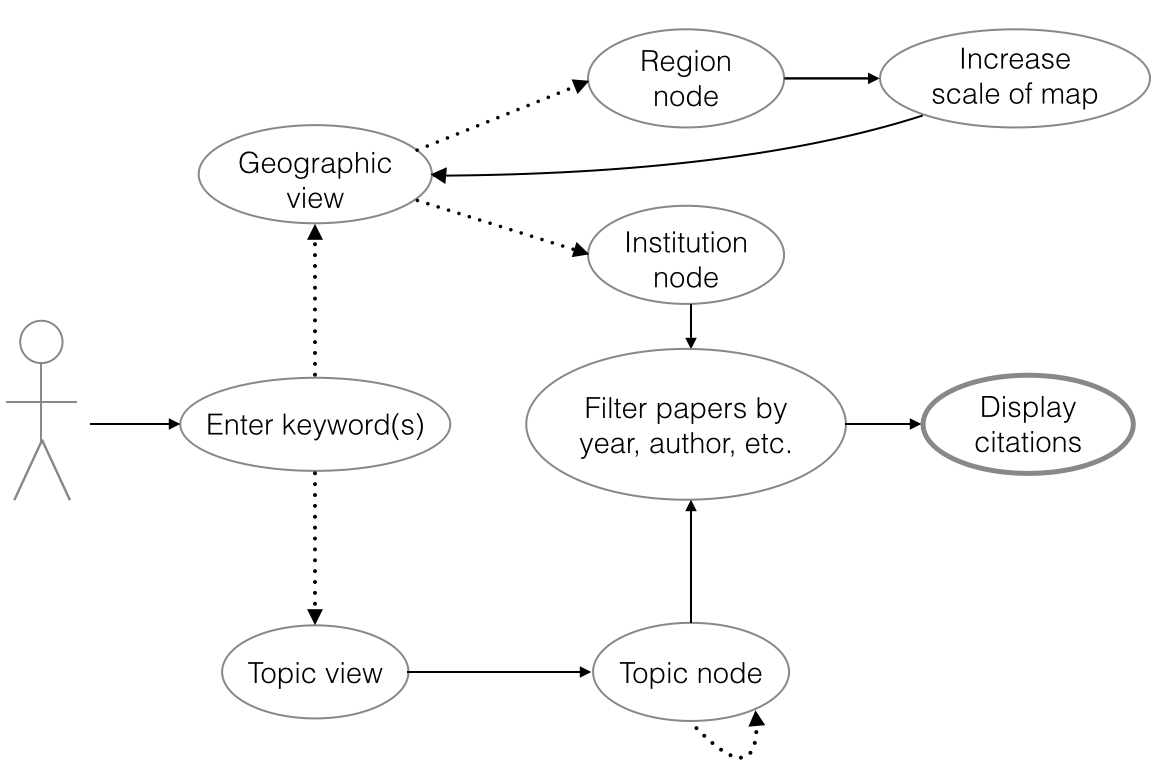
\includegraphics[width=300pt]{../lib/images/user-flowchart}
	\caption{Flowchart of the steps a user is envisioned to take when using the system. There is a single entry point to the system, as an initial query is required to retrieve data and use it to build a visualisation. This can either be viewed according to geographical locations on a world map, or as a cluster diagram categorised by subject headings. The user is then able to refine the dataset by interacting with the different nodes. When the dataset is deemed to be sufficiently specific by the user, filters can be applied in order to display a set of citations.}
\end{figure}\newpage

\section{Objective 1: Semantic Analysis Tools}
\subsection{MeSH terms}
Upon submission of a publication to MEDLINE, authors have the opportunity to attach MeSH terms that characterise the key concepts, biological entities and technologies of note to their work. This manual curation helps direct searches toward relevant citations and can also allow for flexibility in the specificity of terms. As seen in GoPubMed, the terms at the top levels of the hierarchy are extremely broad and are thus associated with a large number of citations. MeSH 2015 has 16 categories\cite{mesh2015} that are organised into tree-like structures, an example of which is shown in Figure 1. The proposed system will filter high-level MeSH terms out of the dataset, and group the remaining terms according to their category.\\

\noindent The MeSH vocabulary is free to download in full, formatted as either XML or ASCII text. A server-side database system for querying MeSH terms has been utilised in previous works\cite{stoyanovich}, the deciding feature of which would be rapid retrieval. As synonyms are represented in document summaries by a list of unique identifiers for other documents, a relational database would be the most efficient method of preserving and utilising these connections. 
	
\subsection{Author keywords}
Due to the dependency of MeSH terms on human time and energy, many publications instead provide keywords that are suggested by the authors. These words are more likely to be variable, producing datasets that are difficult to group efficiently. Unlike MeSH terms, high-level tags are not enforced upon papers so it is largely expected that keywords will be relevant to the topics explored within the publication. Initially, author keywords could be compared to the MeSH vocabulary to see if an exact match can be found. If there is no direct map to a MeSH term, the phrase is presented as a potential new term--appearing in a node of its own. A threshold number of citations would be established to prevent creation of noisy datasets that contain a large number of single-citation nodes. 

\subsection{MetaMap}
The National Library of Medicine has bundled MeSH and a number of other vocabularies and tools to produce a comprehensive set of services termed the Unified Medical Language System (UMLS)\cite{bodenreider}. The most relevant tools for this project are Metathesaurus, a database of BioMedical vocabularies, and MetaMap, a Prolog-based mapping engine\cite{aronson}. In addition to the greater number of concepts and relationships characterised by the UMLS, a higher degree of semantic annotation is accessible when compared to MeSH alone. Many of MetaMaps's features are beyond the scope of this project, however it would be simpler to process MeSH terms and author keywords using the same pipeline, and would likely result in a richer dataset with which to produce a visualisation. The technical disadvantage lies in the access of data via MetaMap. The program is large at 7 GB, and 2 GB of memory is recommended. These requirements are too strenuous for an inexpensive server. Alternatively, the Java API provides access to the mapping engine, the output of which could be parsed as JSON or XML. There is a Clojure wrapper for the 2013v2 API release, which I would be interested in using as I have basic knowledge of Racket, another Lisp dialect. \newpage

\subsection{Deliverables}
There are two clear alternatives for semantic processing of BioMedical keywords, the investigation into which should be carried out early on in the project as it will affect the system architecture. The key milestones in objective 1 are:
\begin{enumerate}
\item{Install MetaMap API, investigate speed and format of output - 3--7 days. If this approach does not appear appropriate:}
	\begin{enumerate}
	\item{Investigate relational database solutions - 1--2 days}
	\item{Download MeSH XML file and enter a small number of records into database - 2--4 days}
	\end{enumerate}
\item{Develop full processing pipeline for document summaries - 1--2 weeks}
\end{enumerate}

\noindent At this stage in the project development of the web framework should begin to ensure that all components are compatible. 

\section{Objective 2: Geocoding of Addresses}
\subsection{Map Technologies}
The geographic view relies on the presentation of the world map in a scalable format. Google Maps (\url{UK, http://maps.google.co.uk/}) and OpenStreetMap (OSM, \url{http://openstreetmap.org/}) are both widely used in both desktop and mobile web applications. OpenStreetMap is initially more appealing, as it is open-source and customisable with alternative tilesets. However, the main feature of interest is the ability of the map service to interpret an address string and return a geographical location, termed \emph{geocoding}\cite{davis}. Upon investigation of searching for institutional addresses on both services, Google was the clear winner (Table 1). The poor coverage of China is a particularly important factor as a large number of papers are published by Chinese researchers. \\

\noindent The Google Places API returns either JSON or XML data in response to sending a HTTP request containing a search string. Since this requires little processing, the requests will be made client-side after normalising the address server-side. The terms and conditions of using the API state that the results must be displayed on Google Maps\cite{google-terms}.

\subsection{Deliverables}
The key milestones in objective 2 are:
\begin{enumerate}
\item{Write script to optimise address strings for the Google Places API - 1--2 weeks}
\item{Ensure that Google Maps can be embedded in the web page - 1--2 days}
\item{Run large number of optimised addresses using API to ascertain success rate - 1--2 days.}
\end{enumerate}\newpage

\begin{landscape}
\begin{savenotes}
\begin{table}[h]
\noindent
\begin{tabular}{ | l | p{6cm} | p{6cm} | }
    \hline
    \bf{Institutional address on PubMed} & \bf{      OSM   Result   (lat,   long)      } & \bf{Google Maps Result (lat, long)}\\ \hline
    Guiyang Medical University, Guiyang, China & n/a & 26.597086, 106.715737\\ 
    Chinese Academy of Sciences, Kunming Yunnan 650223, China & n/a & 25.067471, 102.704811\\ 
    Wenzhou Medical University, Wenzhou, Zhejiang, China & n/a & 27.925146, 120.71201\\ 
    Jiwaji University, Gwalior, India & 26.2043353, 78.1893755 & 26.202972, 78.194203\\ 
    Karolinska Institutet, Stockholm, Sweden & 59.3515453, 18.0310658 & 59.348148, 18.023658\\ 
    Save the Children, Cape Town, South Africa & n/a & -33.970344, 18.46432\footnote{Incorrect location}\\ 
    Faculty of Science, Rangsit University, Pathumthani, Thailand & n/a & 13.9651795, 100.5879664\\ 
    Makerere University, Kampala, Uganda & 0.3343676, 32.5678365 & 0.329183, 32.5709881\\ 
    Malaria Consortium, London, UK & n/a & 51.522621, -0.1072795\\ 
    University of Massachusetts, Amherst, MA, 01003, USA & 42.3889785, -72.5286987 & 42.391157, -72.526712\\ \hline
\end{tabular}
\noindent\caption{Coordinate results from OSM and Google Maps when entering partial global addresses on PubMed. Results were corroborated with addresses found on organisation websites to ensure accuracy.}
\end{table}%
\end{savenotes}
\end{landscape}

\section{Objective 3: Programming Languages and Web frameworks}
\subsection{Python vs. Ruby}
NCBI allows public access to the Entrez databases via a RESTful API, allowing flexibility with programming languages and frameworks due to the universality of the REST. I have chosen to focus on dynamic programming languages as these allow for fast iterative development, which is particularly useful for web applications. I am familiar with Python and Ruby, and each have a multitude of full-stack frameworks and microframeworks to choose from. Python provides comprehensive functionality with modules for sending HTTP requests (urllib and httplib in Python 2 or urllib.request/urllib.parse/urllib.error and http.client in Python 3) and parsing XML (xml.etree.ElementTree) in the standard library. Ruby has modules for HTTP requests, but XML handling requires additional software. Both languages have integrated unit testing libraries, which will be used throughout development. I am keen to learn Python and feel that overall, it is better suited for the task.

\subsection{Flask vs. Django}
At this stage of the project I am unsure of the requirement for large-scale persistence of data, which would sway the decision between full-stack framework and a microframeworks. If I decide to use the MetaMap API, I would prefer to use a microframework, as full-stack frameworks such as Django require a database engine for certain features. This would be useful if I were to create a relational database for MeSH terms instead. Two frameworks of interest are Flask (\url{http://flask.pocoo.org/}) and Django (\url{https://www.djangoproject.com/}), both of which are supportive of RESTful APIs and well-documented. Considering that this project is my first experience in web development, extensive documentation is a priority for choosing a framework, and an active community is also preferred. 

\subsection{Deliverables}
The key milestones in objective 3 are:
\begin{enumerate}
\item{Create skeleton server-side application - 1--2 days} 
\item{Fetch data from the PubMed database - 1--3 days}
\item{Write basic CSS and HTML for front-end - 1--2 weeks}
\item{Integrate MetaMap/MeSH database into framework - 1--2 weeks}
\end{enumerate}

\section{Objective 4: Data Visualisation}
Javascript has become a widely used language for front-end tools and is currently used in 89\% of all websites\cite{w3}. The project requires a rich interactive user interface, for which many front-end JavaScript libraries were developed with in mind.  

\subsection{D3: Data Driven Documents}
D3 (\url{http://d3js.org/}) is an open-source and actively maintained JavaScript library. It is fully-featured with a wide range of built-in functions for manipulating SVG objects, of which Geography and Cluster appear most relevant for this project. Out of the box, D3 appears to have everything required for the project, but if this turns out to not be the case there is a vast collection of specialised plugins and D3-based libraries available from the community. Initially, D3 will be run locally using node.js, and will be implemented in a web browser only if all other objectives have been fulfilled.

\subsection{Deliverables}
The key milestones in objective 4 are:
\begin{enumerate}
\item{Install D3, understand how it works and create basic app from tutorial - 3--5 days}
\item{Incorporate into Google Maps - 3--5 days}
\item{Create visualisations based on a small dataset of keywords - 1--2 weeks}
\item{Investigate if any additional plugins or libraries are required for implementation - 2--3 days}
\item{Ensure that D3 can respond to objects sent from Python framework - 1--2 weeks}
\end{enumerate}

\section{Proposed System Architecture and Usage}
The outline of the system as proposed in the objectives can be organised into server-side for retrieval and processing of results from PubMed, and a client-side for visualisation of the results. This is shown as a diagram in Figure 6, though the exact technologies to be used for assigning semantics to keywords are to be finalised.

\begin{figure}
	\centering
	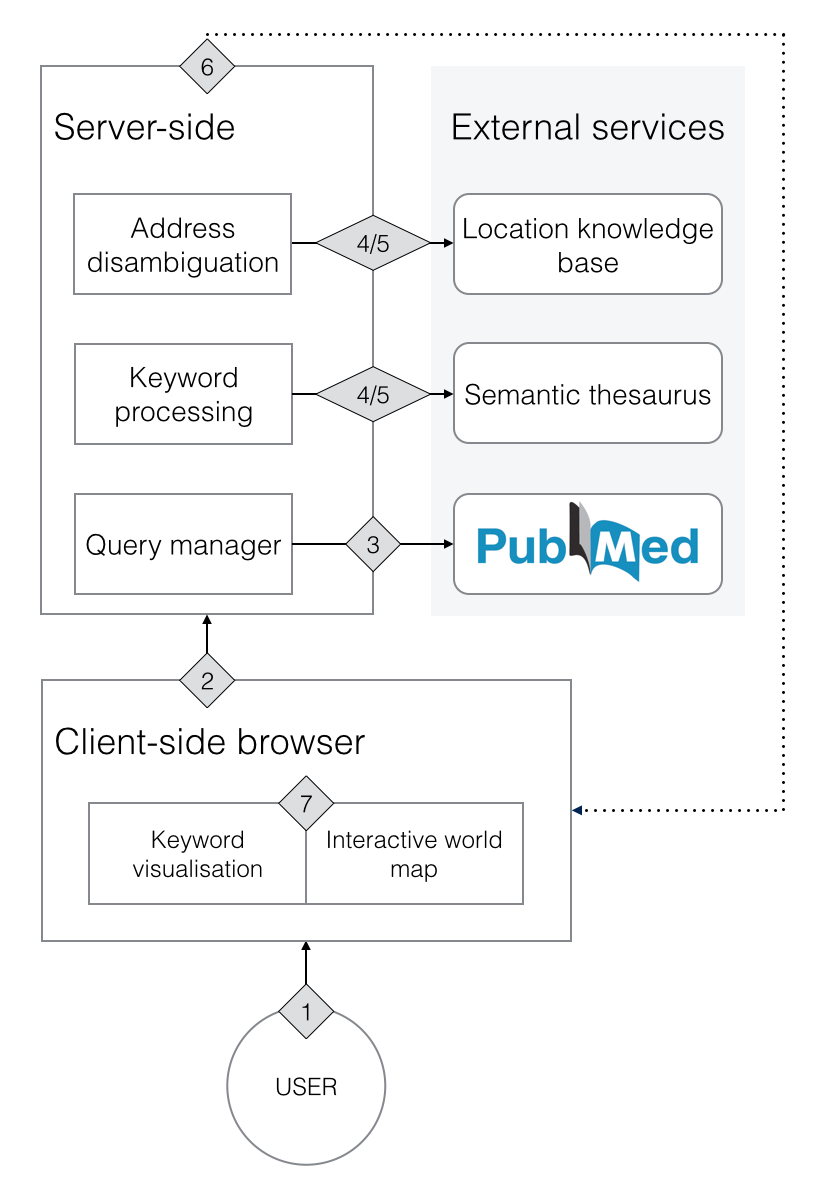
\includegraphics{../lib/images/system-arch}\\
 	\caption{High-level diagram of the structure of and interaction between architecture components. 1. The user interacts with the web application. 2. The query is sent to the server, 3. which sends a GET request to the PubMed database and retrieves the results in XML or JSON format, 4/5. The order of these two stages are interchangeable, as they are concerning different types of data. Keyword processing will be carried out on the fields holding MeSH term and author keywords, using either a locally stored database of MeSH terms or the MetaMap API. Organisation addresses will be normalised to increase the chances of being recognised by the Google Places API. 6. The processed data is sent client-side and 7. a request is sent to the Google Places API to assign geographical coordinates to addresses. 8. Lastly, the results are visualised using D3 and/or Google Maps.}
	\label{fig:SA}
\end{figure}

\end{document}